\section{数值结果与机制讨论}
本节用已有二维计算和预先规定的标量样本解释定理所表达的量，不以有限样本代替总体结论，也不把一条构造攻击当成最坏策略。结果均来自仓库中已保存的数据；本轮没有重新运行仿真或生成随机样本。

\subsection{精确反馈下的真实损伤与双预算界}
二维算例采用
\[
A_{\rm S}=\begin{bmatrix}.82&.18\\-.10&.72\end{bmatrix},\qquad
A_{\rm U}=\begin{bmatrix}1.04&.12\\.03&.91\end{bmatrix},
\]
\[
P_0=\begin{bmatrix}.8&.12\\.12&.6\end{bmatrix},\quad
Q=\begin{bmatrix}.05&.01\\.01&.04\end{bmatrix},\quad
R=\begin{bmatrix}.2&.03\\.03&.3\end{bmatrix},\quad
Z=\begin{bmatrix}2&.25\\.25&1.5\end{bmatrix}.
\]
目标时刻为$k=4$，攻击幅值上限为$b=0.1$。表\ref{tab:damage-decomp}比较持续定向策略与目标拍随机符号、下一拍补偿的合法策略。

\begin{table}[ht]
\centering\footnotesize
\bicaption{真实目标损伤的偏差与协方差分解}{Table \thetable\quad Bias and covariance decomposition of true target damage}
\label{tab:damage-decomp}
\begin{tabular}{llrrr}
\toprule
模型 & 策略 & 偏差能量 & 协方差变化 & 真实损伤$J$\\
\midrule
S & 持续定向 & .001315759 & -.000020445 & .001295314\\
U & 持续定向 & .003252364 & -.000120021 & .003132343\\
S & 两拍符号补偿 & .000321850 & $\simeq0$ & .000321850\\
U & 两拍符号补偿 & .000573797 & $\simeq0$ & .000573797\\
\bottomrule
\end{tabular}
\end{table}

持续策略的协方差变化为负，说明真实MSE增量不等于条件偏差能量；忽略事件历史概率变化会高估这两个例子的损伤。两拍策略在目标前无动作，故目标协方差分布不变。其总体统计上界分别为$0.000457526$和$0.000902386$，对应真实损伤的$1.42$倍和$1.57$倍。事件树结果曾在$b=0.2$下由每组40万次独立重置模拟交叉检查；该检查只核对数值实现，不是定理的依据。

图\ref{fig:budget}展示同一模型在$k=4,b=0.1$下随完整日志TV预算变化的解析界。下界由合法构造给出，上界适用于全部允许攻击；图中不是对$V_{R_{\rm full}}^{(k)}$的数值优化或置信区间。两条界之间的间距反映当前证书的保守程度，不应解释为实际最坏值。

\begin{figure}[ht]
\centering
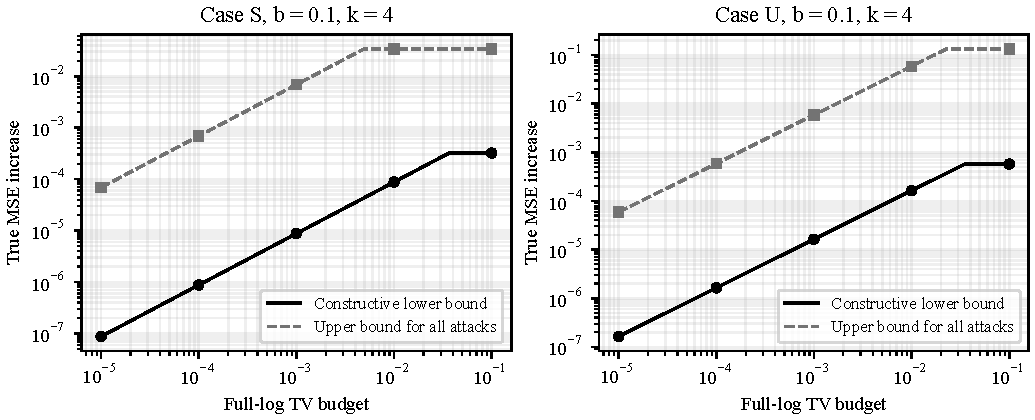
\includegraphics[width=.96\linewidth]{figures/vector_budget.pdf}
\bicaption{固定幅值下的完整日志双预算损伤界（$k=4,b=0.1$）}{Fig. \thefigure\quad Full-log damage bounds under a fixed peak budget ($k=4,b=0.1$)}
\label{fig:budget}
\end{figure}

\subsection{量化反馈下的残余损伤}
标量验证取$A=0.82$（S1）和$A=1.04$（U1），$P_0=0.8$、$Q=0.05$、$R=0.2$、$Z=2$，$k=4$、$b=0.1$。每个模型使用预先固定的2048个独立基础样本，三个量化精度共用配对样本。表\ref{tab:e1-damage}和图\ref{fig:e1}报告B协议中所构造攻击的损伤；它们不是最坏值$V_{R,\delta}^{(k)}$的数值求解。区间为按基础样本配对的探索性bootstrap区间，不是全策略置信界。

\begin{table}[ht]
\centering\footnotesize
\bicaption{B协议中量化见证的目标损伤}{Table \thetable\quad Target damage of the quantized-feedback witness under protocol B}
\label{tab:e1-damage}
\begin{tabular}{lrrrr}
\toprule
模型/精度 & $\delta$ & $10^6\hat J$ & 探索性95\%区间（$10^{-6}$） & $\hat J/\delta^2$\\
\midrule
S1/1 & .00290706 & .295503 & [.256237,.334963] & .034967\\
S1/2 & .00581412 & 1.239223 & [1.086202,1.391006] & .036659\\
S1/3 & .01162823 & 4.814492 & [4.227691,5.429128] & .035606\\
U1/1 & .00556494 & .785686 & [.703663,.878413] & .025370\\
U1/2 & .01112988 & 2.793531 & [2.458229,3.128096] & .022551\\
U1/3 & .02225976 & 11.211802 & [9.942383,12.533812] & .022627\\
\bottomrule
\end{tabular}
\end{table}

本设计令攻击幅值随$\delta$变化且远小于$b$，只覆盖精度主导区。它没有数值检验定理中幅值主导区，也不据三个精度点估计渐近指数。在最大预设精度下，见证损伤约为相应健康MSE的$0.0051\%$（S1）和$0.0077\%$（U1）。这支持“指定遥测下严格零TV保证失效且残余损伤为正”的数学结论，不支持显著工程损害或量化带来正常精度/通信收益的说法。

\begin{figure}[ht]
\centering
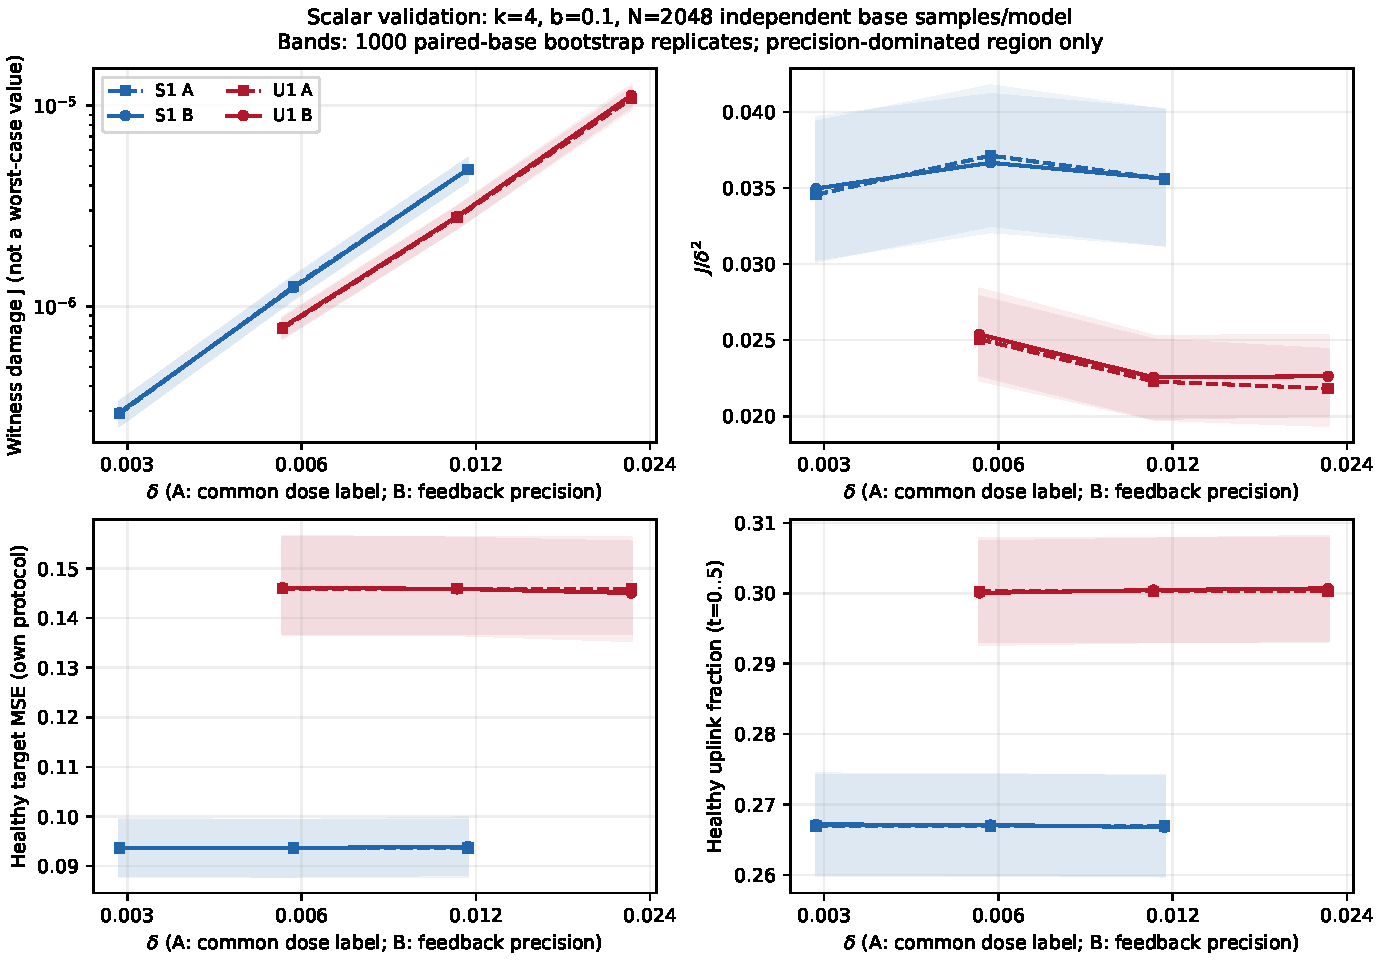
\includegraphics[width=\linewidth]{figures/e1_mechanism.pdf}
\bicaption{量化见证损伤、精度尺度及健康代价}{Fig. \thefigure\quad Quantized-witness damage, precision scaling, and healthy cost}
\label{fig:e1}
\end{figure}

\subsection{记录分辨率与增强审计}
本批A协议每组2048个基础样本均未出现健康与受攻事件串分叉。因此样本事件差为零只反映本次有限样本的分辨率，不能作为总体TV为零的证据；定理中的总体差异由条件概率恒等式支持。相应条件得分差很小，且该诊断使用模拟中的完整条件历史与策略变量，不能解释为审计者已从有限日志中识别出差异。

增强审计C把同一B运行中的连续载荷或未量化预测加入记录。表\ref{tab:e1-c}只列最大预设精度下的代表值：它们与理论矩差一致，足以区分本文构造的独立符号见证，但不证明C能排除所有零TV正损伤策略。对任意攻击，增加字段只给出$V_C\le V_B$。

\begin{table}[ht]
\centering\footnotesize
\bicaption{最大预设精度下增强审计C的代表性矩差}{Table \thetable\quad Representative moment gaps under enhanced audit C at the largest tested precision}
\label{tab:e1-c}
\begin{tabular}{lrr}
\toprule
模型 & 载荷平方差（$10^{-6}$） & 预测平方差（$10^{-6}$）\\
\midrule
S1/3 & 34.445971 & 3.237265\\
U1/3 & 41.684819 & 12.126685\\
\bottomrule
\end{tabular}
\end{table}

综上，二维结果解释了偏差项和协方差项为何必须共同进入真实损伤；预算曲线区分了可达下界与全策略上界；标量结果则说明量化反馈及受限审计记录下的严格隐蔽边界。数值结果没有独立证明一般时域或全部因果策略的结论。
